\documentclass[10pt,twocolumn,letterpaper]{article}

\usepackage{cvpr}
\usepackage{times}
\usepackage{epsfig}
\usepackage{graphicx}
\usepackage{amsmath}
\usepackage{amssymb}
%\usepackage{algorithmic}
\usepackage{algpseudocode}
\usepackage{enumitem}
\usepackage{listings}
\usepackage{amsmath}
\usepackage{algorithm,algpseudocode}
\lstset { %
    language=C++,
    %backgroundcolor=\color{gray!5}, % set backgroundcolor
    basicstyle=\footnotesize,% basic font setting
}



\usepackage{url}

% Include other packages here, before hyperref.

% If you comment hyperref and then uncomment it, you should delete
% egpaper.aux before re-running latex.  (Or just hit 'q' on the first latex
% run, let it finish, and you should be clear).
%\usepackage[pagebackref=true,breaklinks=true,letterpaper=true,colorlinks,bookmarks=false]{hyperref}

\cvprfinalcopy % *** Uncomment this line for the final submission

\def\cvprPaperID{****} % *** Enter the CVPR Paper ID here
\def\httilde{\mbox{\tt\raisebox{-.5ex}{\symbol{126}}}}

% Pages are numbered in submission mode, and unnumbered in camera-ready
\ifcvprfinal\pagestyle{empty}\fi


\newcommand\NoDo{\renewcommand\algorithmicdo{}}
\newcommand\ReDo{\renewcommand\algorithmicdo{\textbf{do}}}
\newcommand\NoThen{\renewcommand\algorithmicthen{}}
\newcommand\ReThen{\renewcommand\algorithmicthen{\textbf{then}}}

\begin{document}

%%%%%%%%% TITLE
\title{K-means in C++/OpenMP/CUDA}

\author{Antonio Castellucci\\
{\tt\small antonio.castellucci@stud.unifi.it}
% For a paper whose authors are all at the same institution,
% omit the following lines up until the closing ``}''.
% Additional authors and addresses can be added with ``\and'',
% just like the second author.
% To save space, use either the email address or home page, not both
\and
Michela Crulli\\
{\tt\small michela.crulli@stud.unifi.it}
}

\maketitle
\thispagestyle{empty}

%%%%%%%%% ABSTRACT

\begin{abstract}

In this report we describe our k-means program structure for image clustering and compare average runtimes of the executions of different implementations: a sequential (in C++) and two parallel implementations (in CUDA and OpenMp). We focused on understanding CUDA and we present our reflections came from experiments done during its learning.
Firstly we define the logic behind the k-means clustering in general and then we define our approach. Afterwards we describe sequential and parallel implementations. We end with the results of the runtimes and the speedups relative to the implementations.
 

\end{abstract}

%%%%%%%%% BODY TEXT
\section{Introduction}

K-means clustering aims to partition input data into k cluster in which each data belongs to the cluster with the nearest mean. K-means algorithm is very popular and used in a variety of applications such as market segmentation, document clustering, image segmentation and image compression. According to the application context, input data can be any type of observations, like pixels of an image.\\
In this section we firstly define k-means clustering from mathematical point of view and later we describe how this clustering technique can be applied to images.
\newpage
\subsection{K-means clustering}

K-Means is an unsupervised learning algorithm and based on centroids. A centroid is a point in features space and it is like a cluster's center of gravity.
For the implementation the first step is to decide the number of cluster in which dataset will be divided. Then K centroids are chosen in the features space. From this point the alghoritm is iterative and the steps are:
\begin{enumerate}
    \item Distance from each point to each centroids is calculated.
    \item Cluster assignment: each point is associated to the cluster with the nearest centroid.
    \item The position of each centroid is recalculated by averaging the positions of all points of the associated cluster.\\
    Formally, given a set of observations (\textbf{x1}, \textbf{x2}, ..., \textbf{xn}), where each observation is a d-dimensional real vector, k-means clustering aims to partition the n observations into k ($\leq$ n) sets \textbf{S} = \{S1, S2, ..., Sk\} so as to minimize the within-cluster sum of squares (WCSS) (i.e. variance).\\
    Therefore, k-means try to minimize the following objective function:

\[J = \sum_{i=1}^k \sum_{x\in S\textsubscript i} || x - \mu \textsubscript i||\textsuperscript 2\]

where $\mu $\textsubscript{i} is the mean of points in S \textsubscript i.

    \item Iterates from step one until in two iteration clusters don't change.
\end{enumerate}

\section{K-means clustering with images}

In our program we have decided to implement k-means applied to images to have a better and immediate correctness verification. For doing this, as shown in the figure below, image pixels are projected from the two dimensional space, with coordinates x, y, related to image grid, into the three dimensional feature space, where the new cordinates are the values of RGB, HSV and others color spaces supported by CImg library that we have used to handle image. K-means is applied to pixels projected in the new feature space with a number of iterations and clusters taken as input from terminal. Ended the last iteration pixels belonging to the same cluster are colored with RGB (or others) values of their cluster centroid.

\begin{figure}[H]
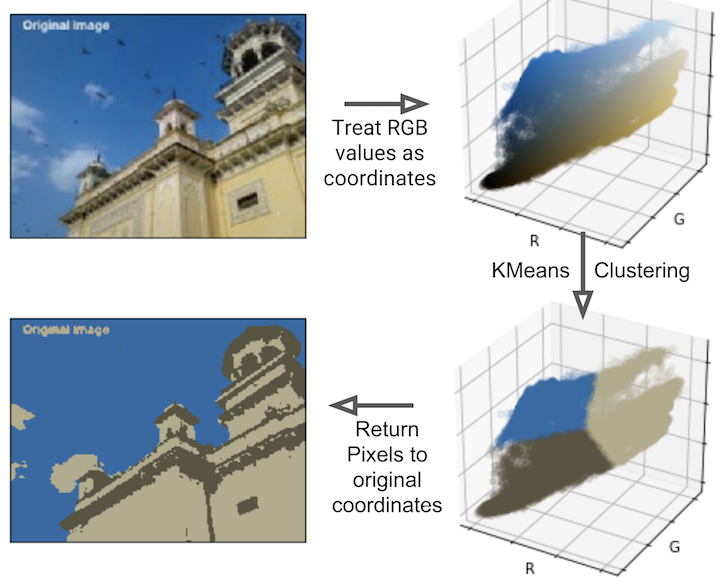
\includegraphics[width=0.4\textwidth]{latex/clustering.png}
\caption{K-means applied to image.}
\label{etichetta}
\end{figure}


\section{Input output structure}

The three different implementation realized are scriptable programs that have the same input/output structure.

\begin{itemize}
    \item Input: \begin{lstlisting}[language=bash]
  $ ./SCRIPT FILE MODE K I [display]
 \end{lstlisting}
    \begin{enumerate}
        \item ./SCRIPT: name of the executable.
        \item FILE: path of the input image.
        \item MODE: mode in which input image (RGB) is converted. User can choose between, RGB, sRGB, HSV, HSI, CMY, HSL.
        \item K: number of cluster in which image is clusterized. Any number from 1 to infinite.
        \item I: number of iterations from 1 to infinite.
        \item display: if this keyword is added, the output change and  the original and clustered images are also displayed, otherwise clusterized image is saved and the execution terminates.
    \end{enumerate}
    
    For example:
    \begin{lstlisting}[language=bash]
  $   ./fastCudaKmeans ./testImage/car.jpg
      RGB 3 500 display
 \end{lstlisting}
  
    \item Output: time of execution is printed in the terminal and the clustered image is saved like:     \begin{lstlisting}[language=bash]
    inputNameCLUSTERIZED.jpg 
 \end{lstlisting}
 If display is set, two windows are displayed as below.
    \begin{figure}[H]
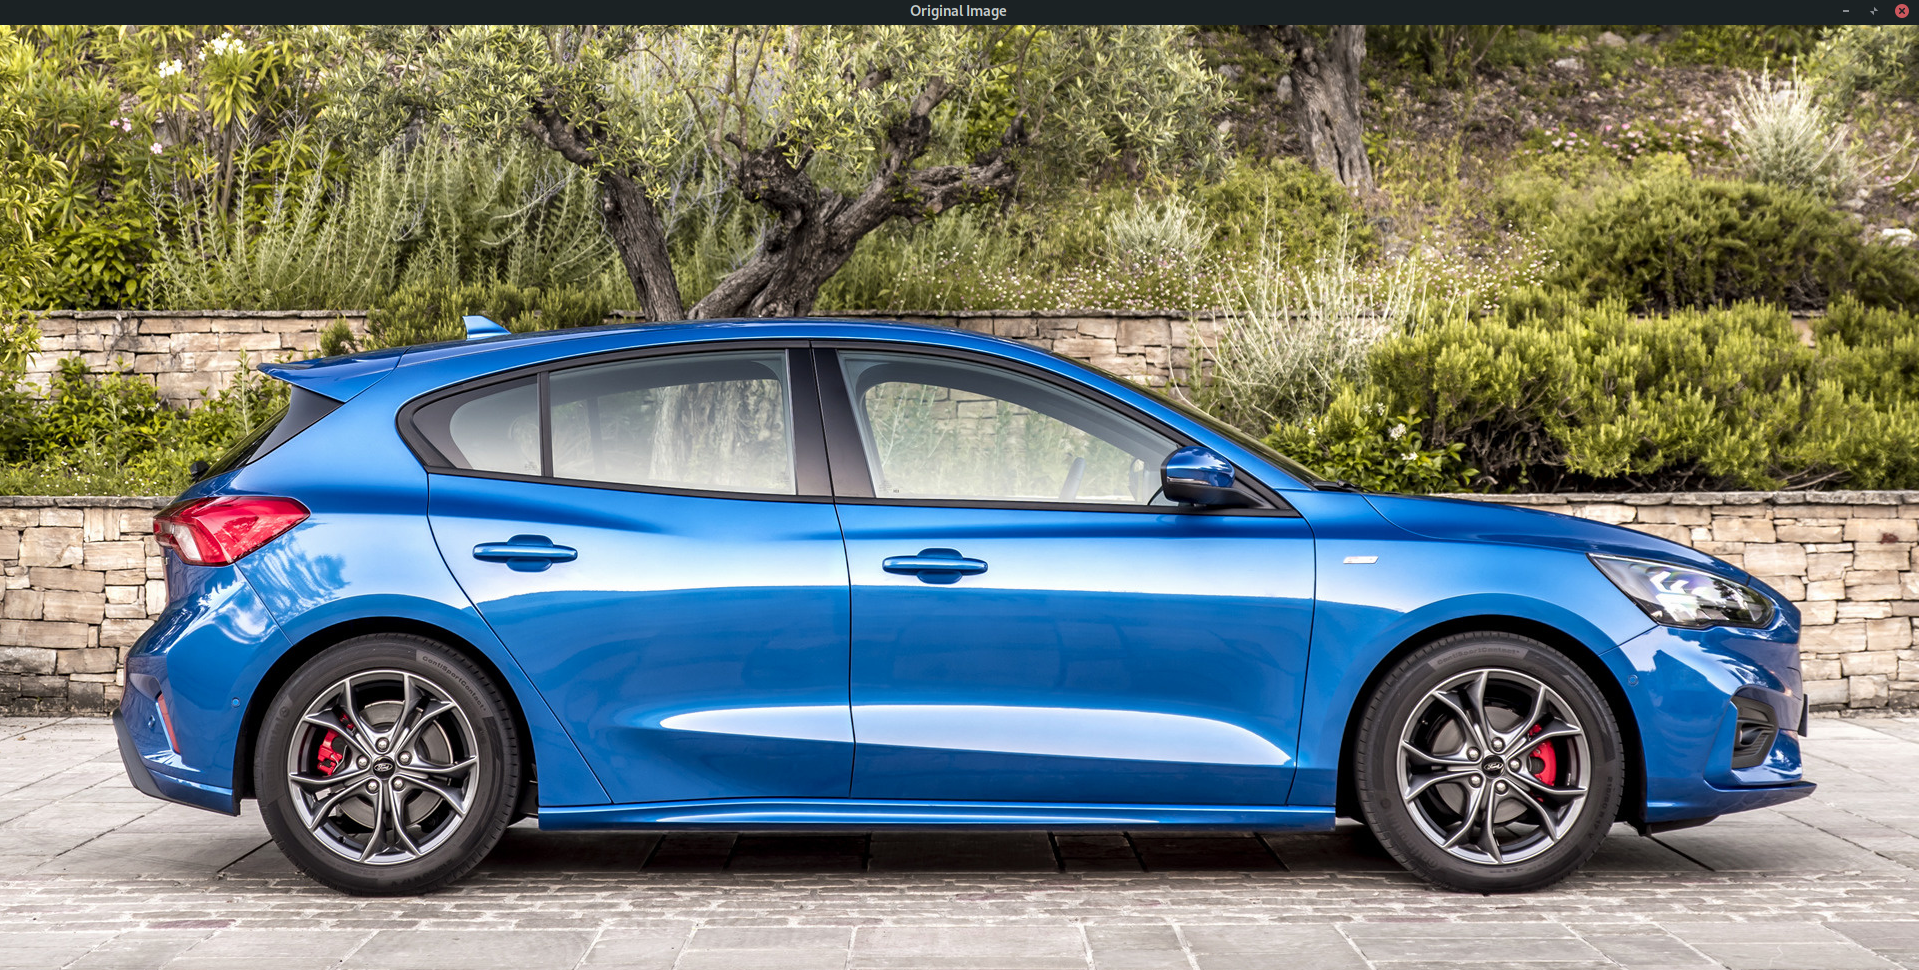
\includegraphics[width=0.22\textwidth]{latex/orig.png}
\hfill
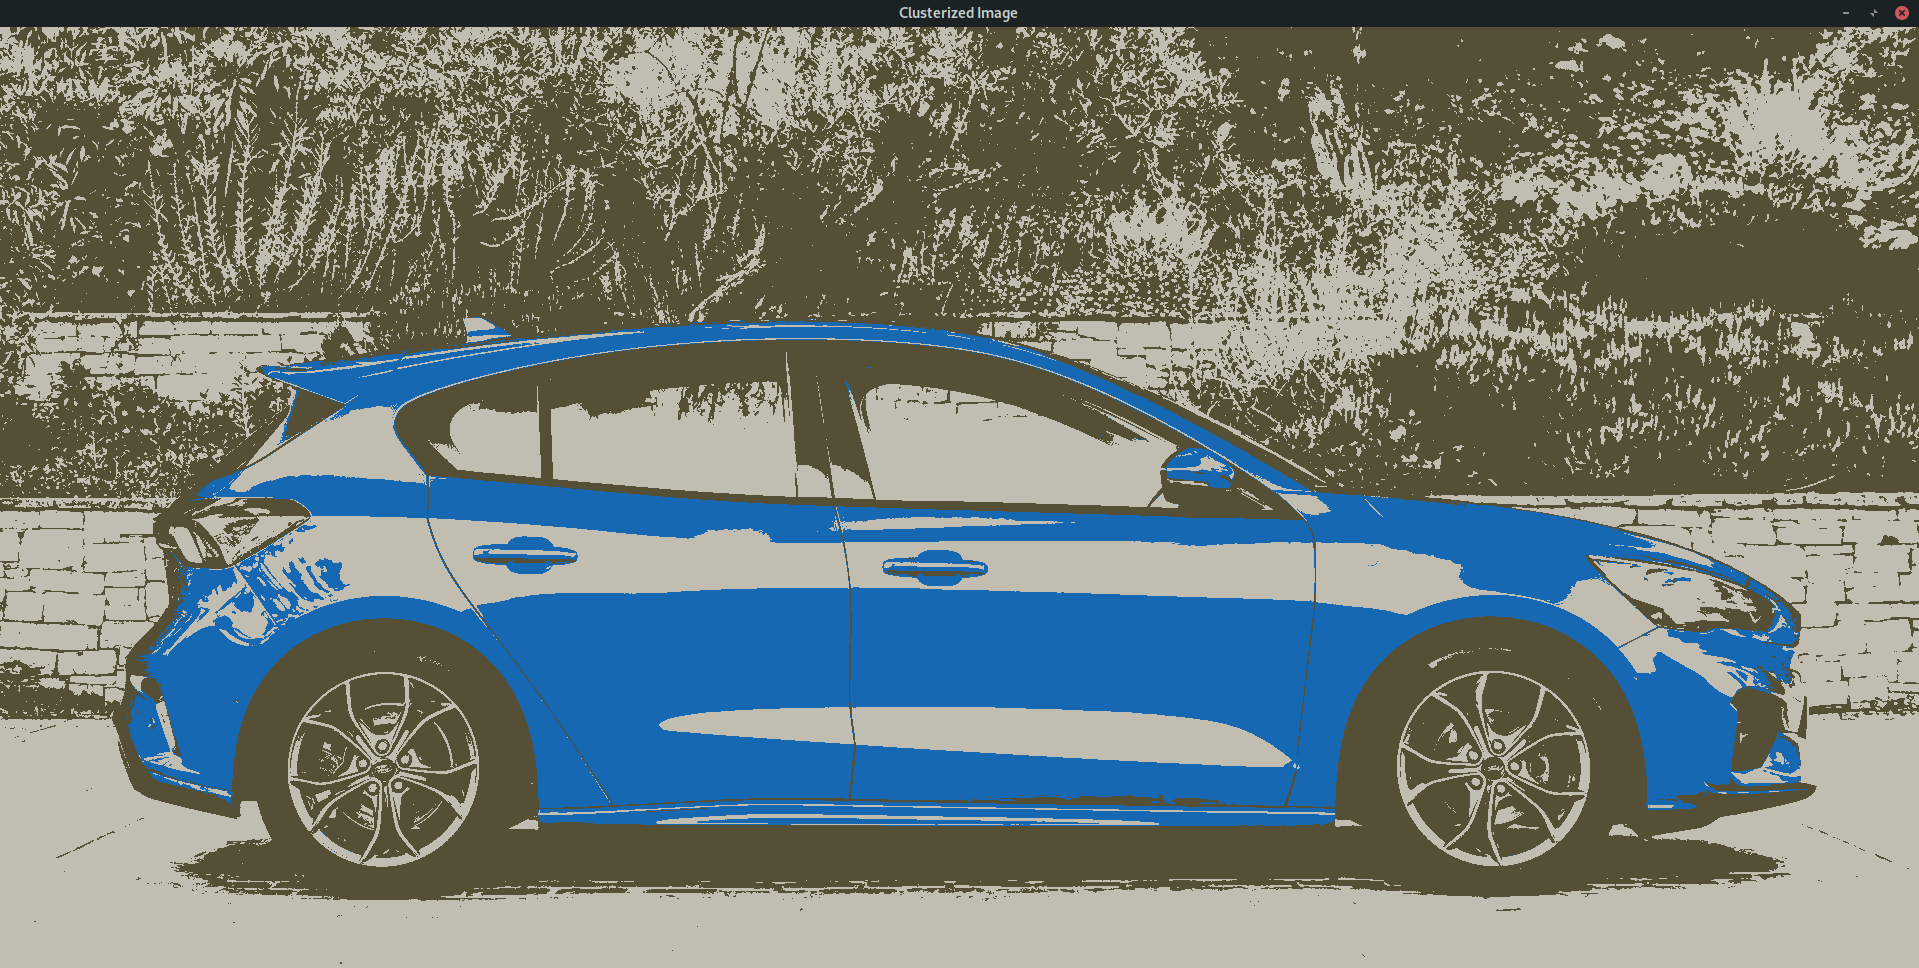
\includegraphics[width=0.22\textwidth]{latex/clust3.png}
\caption{Original and clustered image.}
\label{etichetta}
\end{figure}
\end{itemize}

For the separation of concern and code reusability, different implementations use a common class (ImageHandler) which defines interfaces for pixels values acquisition and processed data elaboration. In section 5.1 we will describe its structure.

\section{Dataset}

Test shown in the  result section uses images of different sizes, we chose these:

\begin{figure}[H]
\begin{minipage}[b]{0.18\textwidth}
\centering
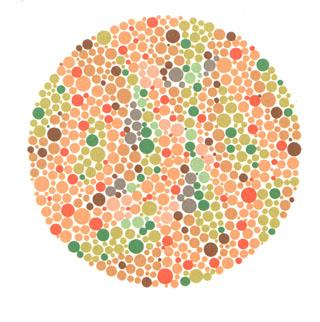
\includegraphics[width=\textwidth]{latex/100000p.jpg}
\caption{10000 pixels.}
\label{etichetta1}
\end{minipage}
\hfill
\begin{minipage}[b]{0.22\textwidth}
\centering
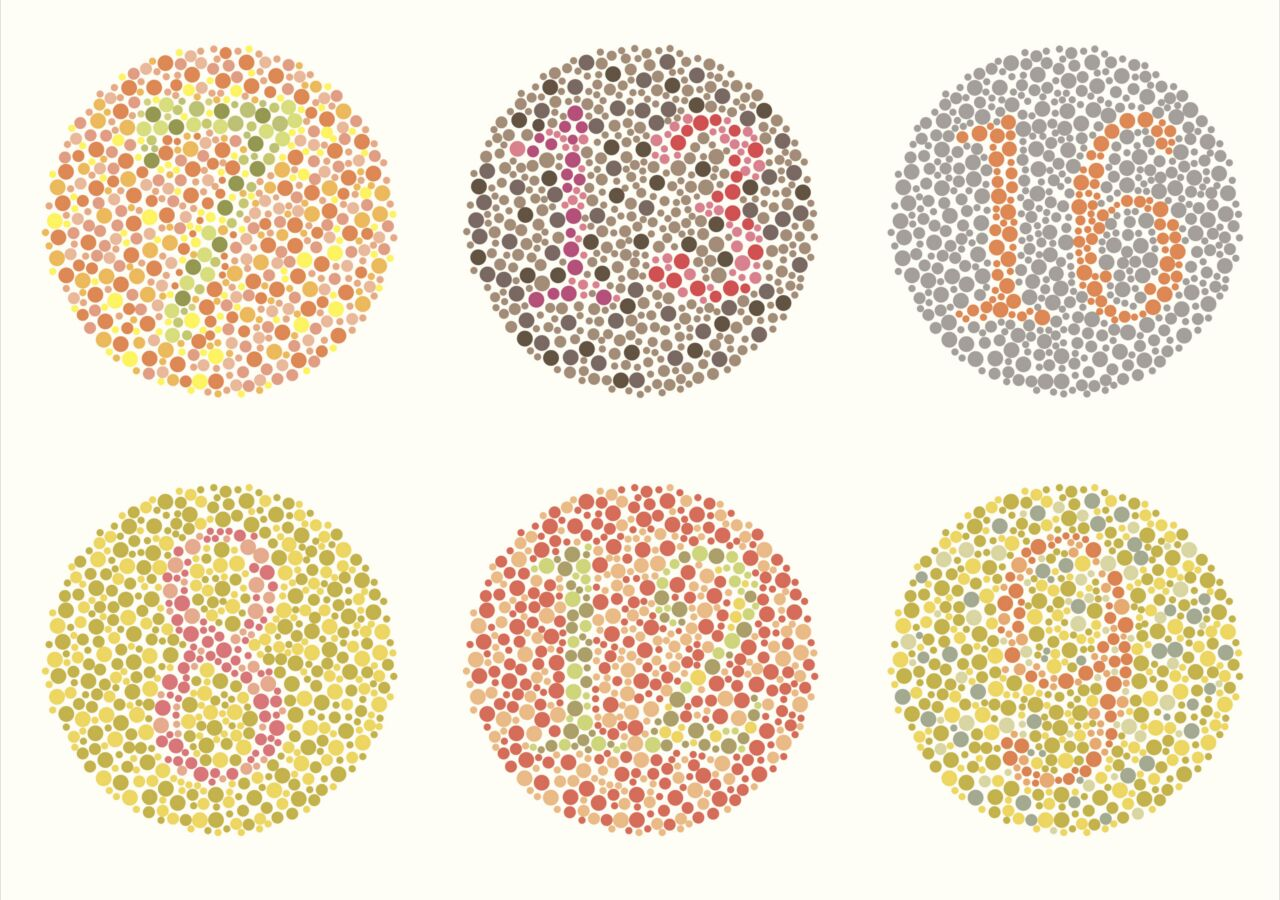
\includegraphics[width=\textwidth]{latex/1Mp.jpg}
\caption{1 millions pixels.}
\label{etichetta2}
\end{minipage}
\hfill
\begin{minipage}[b]{0.22\textwidth}
\centering
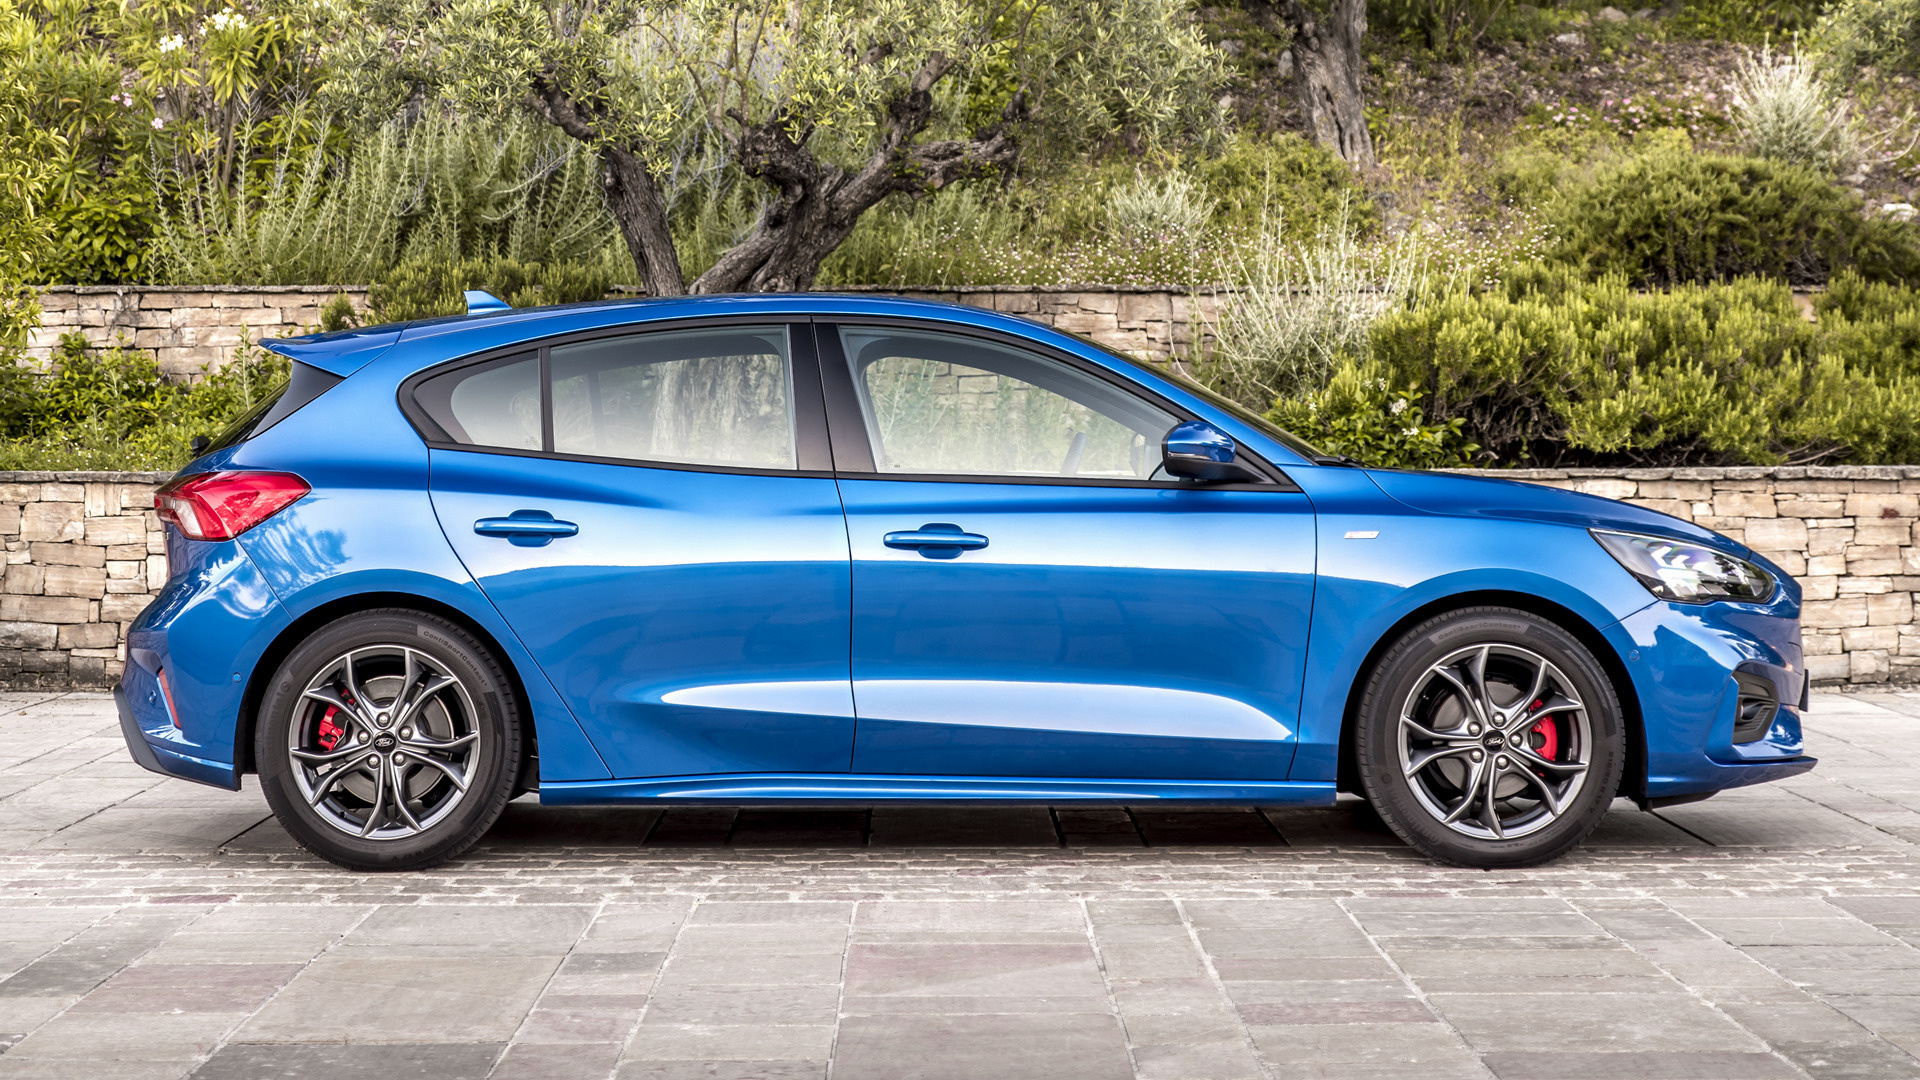
\includegraphics[width=\textwidth]{latex/car.jpg}
\caption{2 millions pixels.}
\label{etichetta2}
\end{minipage}
\hfill
\begin{minipage}[b]{0.22\textwidth}
\centering
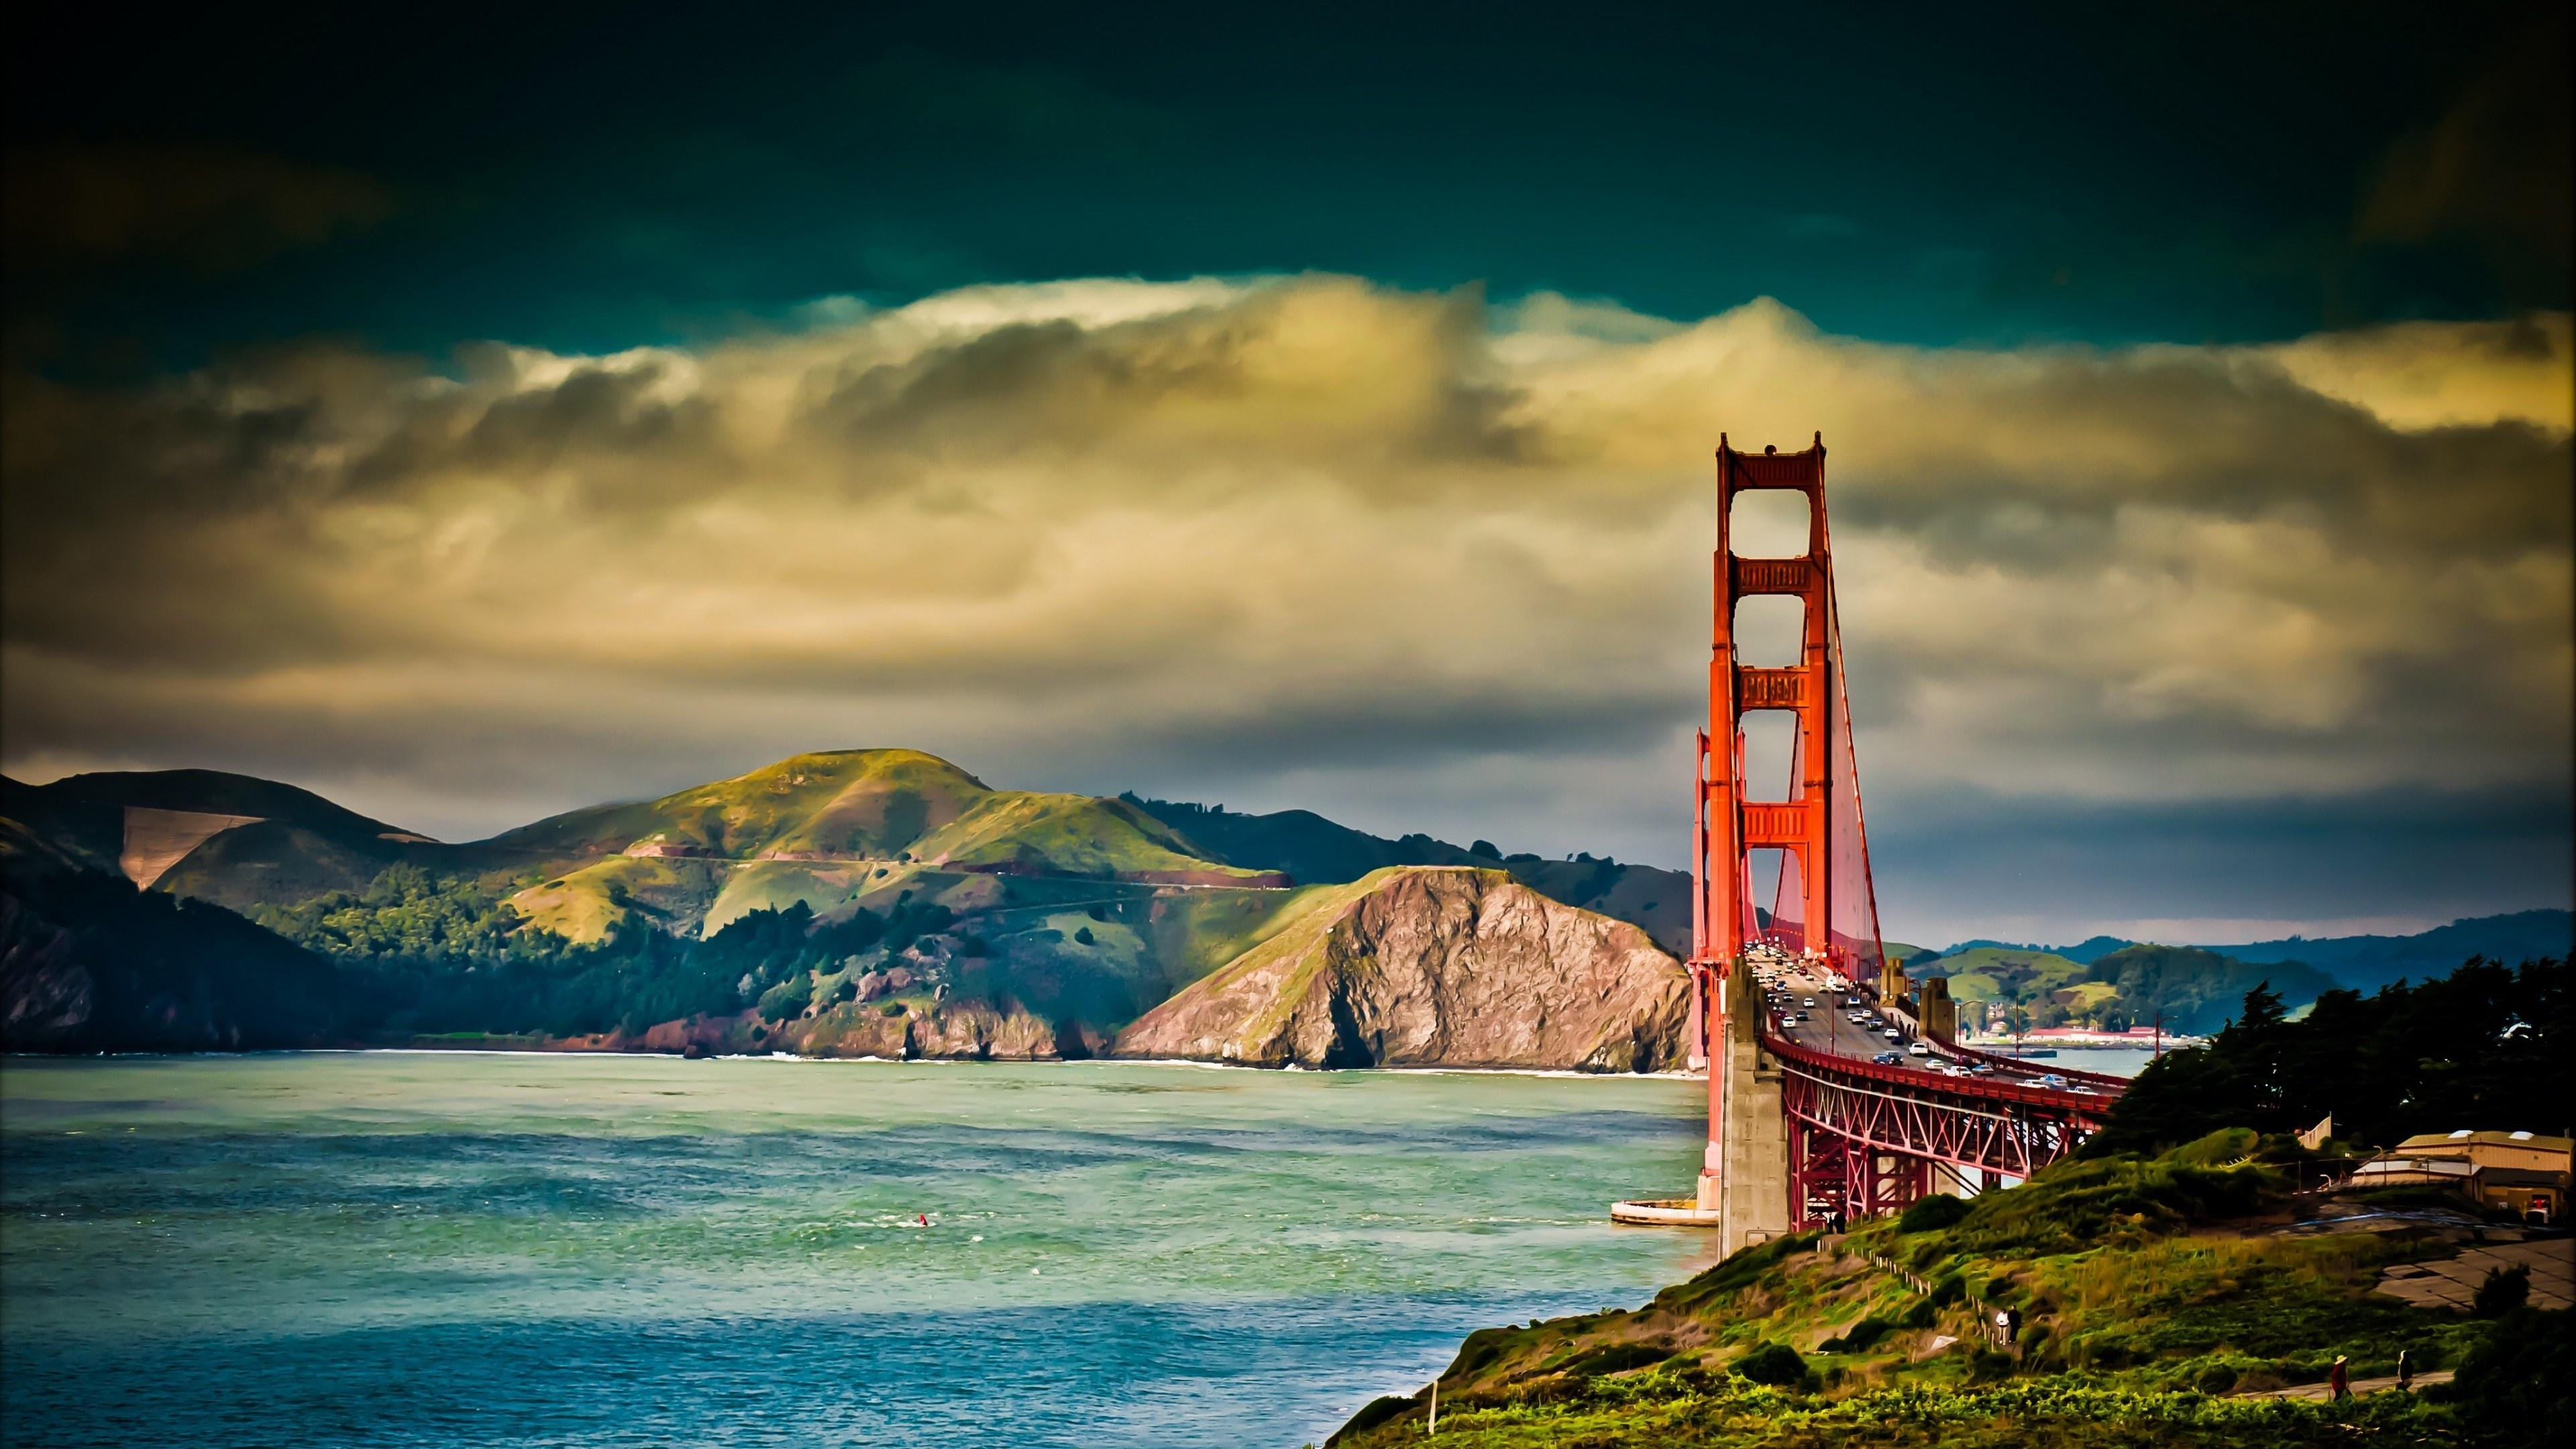
\includegraphics[width=\textwidth]{latex/10Mp.jpg}
\caption{10 millions pixels.}
\label{etichetta2}
\end{minipage}
\end{figure}

\newpage
\section{K-means Implementation}

In this section, we describe more in detail the code structure.
Firstly we describe the common class of the three programs we mentioned before, analysing its attributes, methods and their usage. Then we will go into details of different pseudocodes of k-means.

\subsection{Images Handler}

Now, we describe more in detail the Image Handler class. It’s attributes are:
\begin{itemize}
    \item numberOfClusters: number of clusters in which input image is clusterized.
    \item iterations: the number of iterations.
    \item columns: the width of the input image.
    \item rows: the height of the input image.
    \item filename: the name of the input image.
    \item mode: color space selected, like RGB.
    \item dispImage: command that allows to display the image.
\end{itemize}

While its methods are:
\begin{itemize}
    \item inputParamAcquisition(): takes user input parameters to set class’s attributes and return to main only the number of clusters, iterations, columns, and rows.
    \item dataAcquisition(): takes as input three vectors (one for each feature space coordinates x, y, z) and return these vectors populated with relative pixels values. Vectors are 1-dimensional data structures and their elements position must remain the same for the entire execution because vectors are filled with columns adjacent each other so information about pixel position is encoded without memory usage.
    \item disp(): in this method output image is created and if display option has been set, by command line, the output image is also displayed (not only saved in same input image folder). For making the output this method takes in input a vector that, for each pixel, indicates the cluster it belongs to and three smaller vectors filled with clusters means values.
\end{itemize}
\begin{figure}[H]
\begin{center}
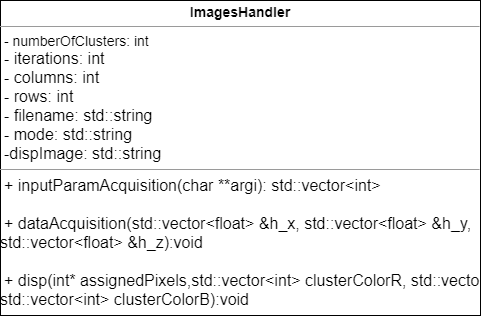
\includegraphics[width=0.4\textwidth]{latex/IMageHANDLERuml.png}
\caption{ImagesHandler UML}
\label{etichetta}
\end{center}
\end{figure}

In the figure above there is the methods and attributes of the class just described. 
Now, in the figure below, we will see how this class interacts with the main of the three programs.
\begin{figure}[H]
\begin{center}
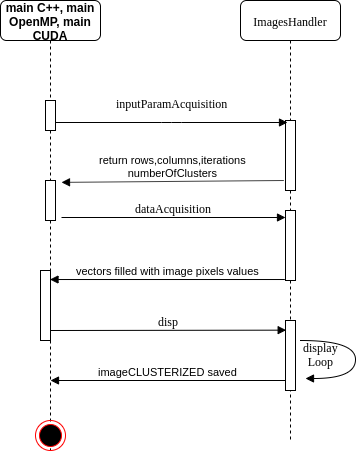
\includegraphics[width=0.32\textwidth]{latex/ImageHandlerIteractions.png}
\caption{Sequence diagram of interaction between ImagesHandler and different k-means implementations}
\label{etichetta}
\end{center}
\end{figure}

\newpage
\subsection{Sequential implementation: C++}

The Sequential implementation of k-means clustering computes, for all iterations and for all pixels of input image, the distances between all points and all clusters and every time a distance is lower than  best distance for the current point, updates the best distance and best cluster. Once all points have their best clusters ID saved into the relative assignment vector position, two loops compute the new clusters means for next iteration.

\algdef{SE}[FOR]{NoDoFor}{EndFor}[1]{\algorithmicfor\ #1}{\algorithmicend\ \algorithmicfor}%
\algdef{SE}[IF]{NoThenIf}{EndIf}[1]{\algorithmicif\ #1}{\algorithmicend\ \algorithmicif}%
\begin{algorithm}[H]
  \caption{c++}\label{alg1}
  \begin{algorithmic}[1]
   \State \textbf{Input:} data, number\_of\_cluster, number\_of\_iterations
    \State \textbf{Output:} means, data.assignments
    \NoDoFor{ i=0 to number\_of\_cluster}
    \State centroids population in means[i]
    \EndFor
    \NoDoFor{iteration = 0 to number\_of\_iterations}
        \NoDoFor{point = 0 to data.size()}
            \State $best\_distance = d(data[point],means[0])$
            \State $best\_cluster = 0$
            \NoDoFor{cluster = 1 to number\_of\_cluster}
                \State $dist = d(data[point], means[cluster])$
                \NoThenIf{dist $<$ best\_distance}
                    \State $best\_distance = dist$
                    \State $best\_cluster = cluster$
                \EndIf
                \EndFor
            \State $data.assignments[point] = best\_cluster$
        \EndFor
        \NoDoFor{point = 0 to data.size()}
            \State $cluster = data.assignments[point]$
            \State $new[cluster].x += data[point].x$
            \State $new[cluster].y += data[point].y$
            \State $new[cluster].z += data[point].z$
            \State $counts[cluster] += 1$
        \EndFor
        \NoDoFor{cluster = 0 to number\_of\_cluster}
            \State $count = counts[cluster]$
            \State $means[cluster].x = new[cluster].x/count$
            \State $means[cluster].y = new[cluster].y/count$
            \State $means[cluster].z = new[cluster].z/count$
        \EndFor
    \EndFor
  \end{algorithmic}
\end{algorithm}

\subsection{Parallel implementation: OpenMP}

Now we can see the first parallel version of k-means clustering using OpenMP framework. OpenMp directive generates code at compile time that allows to parallelize the outer for loop. "parallel for" is a special construct that divide loop blocks to all threads involved. It is possible to use dynamic or static scheduling , and use a chunck argument, to set the size of each block, in each one.
\begin{itemize}
    \item Static iterations are divided into chuncks of size chunck\_size. When no chunck\_size is specified, the iteration space is divided into chuncks that are approximately equal in size or as equal as possible where the number of loop iterations is not evenly divisible by the number of threads multiplied by the chunk size.
    \item In dynamic each thread executes a chunk of iterations, then requests another chunk, until no chunks remain to be distributed. By default the chunk size per block of loop iterations is set to 1.
    
\end{itemize}

\algdef{SE}[FOR]{NoDoFor}{EndFor}[1]{\algorithmicfor\ #1}{\algorithmicend\ \algorithmicfor}%
\algdef{SE}[IF]{NoThenIf}{EndIf}[1]{\algorithmicif\ #1}{\algorithmicend\ \algorithmicif}%
\begin{algorithm}[H]
    \caption{openMP}\label{alg1}
    \label{alg:algorithm_sum}
    \begin{algorithmic}[1]
       \State \textbf{Input:} data, number\_of\_cluster, number\_of\_iterations
        \State \textbf{Output:} means, data.assignments
        \NoDoFor{ i=0 to number\_of\_cluster}
        \State centroids population in means[i]
        \EndFor
        \NoDoFor{iteration = 0 to number\_of\_iterations}
            \State \#pragma omp parallel for
            \NoDoFor{point = 0 to data.size()}
                \State {$best\_distance = d(data[point],means[0])$}
                \State $best\_cluster = 0$
                \NoDoFor{cluster = 0 to number\_of\_cluster}
                    \State $dist = d(data[point],means[cluster])$
                    \NoThenIf{dist $<$ best\_distance}
                        \State $best\_distance= dist$
                        \State $best\_cluster = cluster$
                    \EndIf
                \EndFor
            \State $data.assignments[point] = best\_cluster$
        \EndFor
        \NoDoFor{point = 0 to data.size()}
            \State $cluster = data.assignments[point]$
            \State $new[cluster].x += data[point].x$
            \State $new[cluster].y += data[point].y$
            \State $new[cluster].z += data[point].z$
            \State $counts[cluster] += 1$
        \EndFor
        \State \#pragma omp parallel for
        \NoDoFor{cluster = 0 to number\_of\_cluster}
            \State $count = counts[cluster]$
            \State $means[cluster].x = new[cluster].x/count$
            \State $means[cluster].y = new[cluster].y/count$
            \State $means[cluster].z = new[cluster].z/count$
        \EndFor
    \EndFor
  \end{algorithmic}
\end{algorithm}

  Because distances computations are independent of each other we can parallelize them.
    While, if we parallelize the updating of cluster averages, we have a race condition. We have tried \#pragma omp critical or \#pragma omp atomic to avoid race condition but we had a deterioration in performance so great that we decided to leave the section sequential.
    The best solution is to use \#pragma omp reduction, but in our code we use c++ structs and openMP doesn't support reduction with them.
\subsection{Cuda implementation: Naive}

The approach we initially had, was to replicate the same algorithm used in the others implementations, adapting it to NVIDIA technology.
Thanks to the huge number of threads available on GPUs, we parallelized the first phase of k-means, assigning one pixel to each thread.
A single thread calculates the distance between its point and all clusters.
This is done into assign\_cluster kernel function which uses shared memory to speed up access to the values of the cluster averages. The use of global memory for this first phase results in a speedup of X0.5.
Once the thread has found the best cluster for its point, it uses a slow but simple atomicAdd to adding three RGB values of its pixel to the new average of the best cluster and increase by 1 the new number of elements belonging to the best cluster.
When all the points have been reassigned, a second kernel function takes care of launching one thread for each cluster which divides the RGB values of the cluster (which are equal to the sum of the RGB values of all the points belonging to the cluster) by the number of pixels that belong to it.
This solution efficiently parallelizes the calculation of distances but not the calculation of the new averages, so we looked for a more efficient solution.\\

\algdef{SE}[FOR]{NoDoFor}{EndFor}[1]{\algorithmicfor\ #1}{\algorithmicend\ \algorithmicfor}%
\algdef{SE}[IF]{NoThenIf}{EndIf}[1]{\algorithmicif\ #1}{\algorithmicend\ \algorithmicif}%
\algdef{SE}[DOWHILE]{Do}{doWhile}{\algorithmicdo}[1]{\algorithmicwhile\ #1}%
\begin{algorithm}[H]
    \caption{cudaKmeans}
    \label{alg:algorithm_sum}
    \begin{algorithmic}[1]
        \State{\textbf{Input:} data, k=number\_of\_cluster,number\_of\_iterations}
        \State{\textbf{Output:} means, data.assignments}
        \NoDoFor{i=0 to k}
            \State {centroids population in means[i]}
        \EndFor
        \NoDoFor{iteration = 0 to number\_of\_iterations}
            \State{$assign\_cluster(data, means, k, new\_sums)$}
            \State{$cudaDeviceSynchronize()$}
            \State{$compute\_new\_means(means, new\_sums)$}
            \State{$cudaDeviceSynchronize()$}
        \EndFor
    \end{algorithmic}
\end{algorithm}



\algdef{SE}[FOR]{NoDoFor}{EndFor}[1]{\algorithmicfor\ #1}{\algorithmicend\ \algorithmicfor}%
\algdef{SE}[IF]{NoThenIf}{EndIf}[1]{\algorithmicif\ #1}{\algorithmicend\ \algorithmicif}%
\algdef{SE}[DOWHILE]{Do}{doWhile}{\algorithmicdo}[1]{\algorithmicwhile\ #1}%
\begin{algorithm}[H]
    \caption{compute\_new\_means}
    \label{alg:algorithm_sum}
    \begin{algorithmic}[1]
        \State{\textbf{Input:} means, new\_sums}
        \State{\textbf{Output:} means}
        \State cluster = threadIdx.x
        \State means.x[cluster] = new\_sum.x[cluster] / counts[cluster]
        \State means.y[cluster] = new\_sum.y[cluster] / counts[cluster]
        \State means.z[cluster] = new\_sum.z[cluster] / counts[cluster]
    \end{algorithmic}
\end{algorithm}


\algdef{SE}[FOR]{NoDoFor}{EndFor}[1]{\algorithmicfor\ #1}{\algorithmicend\ \algorithmicfor}%
\algdef{SE}[IF]{NoThenIf}{EndIf}[1]{\algorithmicif\ #1}{\algorithmicend\ \algorithmicif}%
\algdef{SE}[DOWHILE]{Do}{doWhile}{\algorithmicdo}[1]{\algorithmicwhile\ #1}%
\begin{algorithm}
    \caption{assign\_cluster}
    \label{alg:algorithm_sum}
    \begin{algorithmic}[1]
   \State \textbf{Input:} data, means, new\_sums, k
    \State \textbf{Output:} data
    \State index = blockIdx.x * blockDim.x + threadIdx.x
    \NoThenIf{index $\geq$ data\_size} return
    \EndIf
    \State best\_distance = d(data[index],means[0])
    \State best\_cluster = 0
    \NoDoFor{cluster = 1 to k}
        \State $distance = d(data[index],means[cluster])$
        \NoThenIf{distance $<$ best\_distance}
            \State $best\_distance = distance$
            \State $best\_cluster = cluster$
        \EndIf
    \EndFor
     \State data.assignments[index]=best\_cluster
     \State atomicAdd(new\_sums.x[best\_cluster],data.x[point])
	 \State atomicAdd(new\_sums.y[best\_cluster], data.y[point])
	\State atomicAdd(new\_sums.z[best\_cluster], data.z[point])
	\State atomicAdd(counts[best\_cluster], 1)
  \end{algorithmic}
\end{algorithm}
\newpage
\subsection{Cuda k-means with reduction}
Since the computation of a cluster average can be seen as h sums (where h is the number of elements belonging to the cluster) and a single division (by the number of cluster elements), we have tried to implement the reduction.\\
\textit{Reduction} is a common operation for adding up a long array of numbers. One simple implementation of a reduction kernel (run on the CPU) might look like this in C++:

  \begin{lstlisting}
   float reduction(float* A, site_t N){
        float result=0;
        for(size_t i = 0; i < N; i++){
            result += A[i];
        return result;
        }
    }
    \end{lstlisting}

If we have a very large N, this can get quite slow, we want to parallelize this operation. If we’re on a single CPU, with 8 threads, this can be fairly straightforward: divide the array in 8 parts, have the 8 threads sum up their elements, and finally sum up the 8 partial results. Classic divide-and-conquer.\\
On a GPU however, we have thousands of threads subdivided into (potentially) hundreds of blocks. If we want to obtain maximum performance, we need to be careful about how we go about divvying up the workload among blocks, and how we sum up partial results.

\begin{figure}[H]
\begin{center}
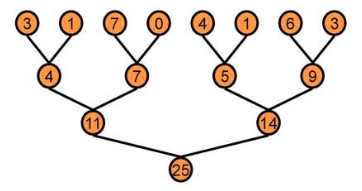
\includegraphics[width=0.3\textwidth]{latex/red.png}
\caption{Tree-based approach used within each thread block.}
\label{etichetta}
\end{center}
\end{figure}

Each thread block reduces a portion of the array but how partial results between thread blocks communicate?\\
If we could synchronize across all thread blocks, could easily reduce very large arrays. Global sync after each block produces its result, once all blocks reach sync, continue recursively but CUDA has no global synchronization because it is expensive to build in hardware for GPUs with high processor count and would force programmer to run fewer blocks (no more than \# multiprocessors * \# resident blocks/multiprocessor) to avoid deadlock, which may reduce overall efficiency.\\
The solution is to divide into multiple kernels: Kernel launch serves as a global synchronization point and it has negligible HW overhead, low SW overhead.

\begin{figure}[H]
\begin{center}
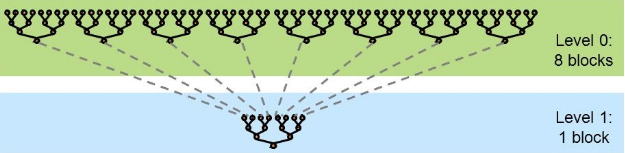
\includegraphics[width=0.47\textwidth]{latex/red1.png}
\caption{Avoid global sync by decomposing computation into multiple kernel invocations.}
\label{etichetta}
\end{center}
\end{figure}

In the case of reductions, code for all levels is the same and it is possible to do Recursive kernel invocation.\\
Mark Harris of Nvidia made a deep dive into how to optimize a CUDA reduction kernel and we tried to implement some of his tricks.

\begin{lstlisting}
template <size_t blockSize> 
__device__ void warpReduce(volatile int *sdata,
                            size_t tid) { 
if (blockSize >= 64) sdata[tid] += sdata[tid + 32]; 
if (blockSize >= 32) sdata[tid] += sdata[tid + 16]; 
if (blockSize >= 16) sdata[tid] += sdata[tid + 8]; 
if (blockSize >= 8) sdata[tid] += sdata[tid + 4]; 
if (blockSize >= 4) sdata[tid] += sdata[tid + 2]; 
if (blockSize >= 2) sdata[tid] += sdata[tid + 1]; 
}

template <size_t blockSize> 
__global__ void reduce(int *g_idata, int *g_odata, 
                        unsigned int n) {
                        
extern __shared__ int sdata[]; 
unsigned int tid = threadIdx.x; 
unsigned int i = blockIdx.x * (blockSize * 2) + tid; 
unsigned int gridSize = blockSize * 2 * gridDim.x; 
sdata[tid] = 0; 

while (i < n) { 
    sdata[tid] += g_idata[i] + g_idata[i+blockSize]; 
    i += gridSize; 
} 
__syncthreads(); 
if (blockSize >= 1024) {
    if (tid < 512) { 
        sdata[tid] += sdata[tid + 512];
    } __syncthreads(); } 
if (blockSize >= 512) { 
    if (tid < 256) { 
        sdata[tid] += sdata[tid + 256];
    } __syncthreads(); } 
if (blockSize >= 256) { 
    if (tid < 128) { 
        sdata[tid] += sdata[tid + 128];
    } __syncthreads(); } 
if (blockSize >= 128) {
    if (tid < 64) { 
        sdata[tid] += sdata[tid + 64]; 
    } __syncthreads(); } 
if (tid < 32) warpReduce<blockSize>(sdata, tid); 
if (tid == 0) g_odata[blockIdx.x] = sdata[0];
} 

\end{lstlisting}

The code above summarizes the reduction for a single vector (in our algorithm there are four) and below we analyze some of the solutions implemented providing reasons behind them.

\begin{itemize}
    \item Urolling loops: If we knew the number of iterations at compile time, we could completely unroll the reduction. The block size is limited by the GPU to 1024 threads so we can easily unroll for a fixed block size but we need to be generic. Templates are the solution, indeed CUDA supports C++ template parameters on device and host functions.This technique solves the waste of resources common to all addressing practices: interleaved addressing and sequential addressing .\\
    In the code appears warpReduce : As reduction proceeds, $#$ “active” threads decreases and when n $<$= 32, we have only one warp left. Instructions are SIMD synchronous within a warp, that means when n $<$= 32 there is no need to \_\_syncthreads(), no need “if (tid $<$ n)” because it doesn’t save any work and it is possible to unroll the last 6 iterations of the inner loop.
    \item Multiple adds/threads: If we init shared memory like this:
    \begin{lstlisting}
    for (unsigned int s=blockDim.x/2; s>0; s>>=1) { 
        if (tid < s) { 
            sdata[tid] += sdata[tid + s]; 
        } 
        __syncthreads();
    } 
    \end{lstlisting}
    
    Half of the threads are idle on first loop iteration and  this is wasteful. Mark Harris suggest to do two loads and a first add of the reduction:
    \vspace{-0.1cm}  
\begin{lstlisting}
unsigned int tid = threadIdx.x; 
unsigned int i = blockIdx.x*(blockDim.x*2)
                + threadIdx.x; 
sdata[tid] = g_idata[i] 
            + g_idata[i + blockDim.x];

__syncthreads();
\end{lstlisting}

    Or better a while loop to add as many elements as necessary:
    \vspace{-0.1cm}  
    \begin{lstlisting}
    unsigned int tid = threadIdx.x; 
    unsigned int i = blockIdx.x*(blockSize*2) 
                    + threadIdx.x; 
    unsigned int gridSize = blockSize*2
                            *gridDim.x; 
    sdata[tid] = 0; 
    while (i < n) { 
        sdata[tid] += g_idata[i] 
                    + g_idata[i + blockSize]; 
        i += gridSize; 
    }
    __syncthreads();
    
    \end{lstlisting}
\end{itemize}
\vspace{-0.4cm} 
Reduction merely adds array elements and now we illustrate how we have applied to k-means centroid update step.
\algdef{SE}[FOR]{NoDoFor}{EndFor}[1]{\algorithmicfor\ #1}{\algorithmicend\ \algorithmicfor}%
\algdef{SE}[IF]{NoThenIf}{EndIf}[1]{\algorithmicif\ #1}{\algorithmicend\ \algorithmicif}%
\algdef{SE}[DOWHILE]{Do}{doWhile}{\algorithmicdo}[1]{\algorithmicwhile\ #1}%
\begin{algorithm}[H]
    \caption{fastCudaKmeans 1.0}
    \label{alg:algorithm_sum}
    \begin{algorithmic}[1]
        \State{\textbf{Input:} data, k=number\_of\_cluster,number\_of\_iterations}
        \State{\textbf{Output:} processed data}
        \NoDoFor{i=0 to k}
            \State {centroids population in means[i]}
        \EndFor
        \NoDoFor{iteration = 0 to number\_of\_iterations}
            \State{$assign\_cluster(data, means, k)$}
            \State{$cudaDeviceSynchronize()$}
            \NoDoFor{cluster = 0 to k}
                \State{ $populate(data, clusterData, cluster)$}
                \State{ $cudaDeviceSynchronize()$}
                \State{ $n = number\_of\_pixels$}
                \Do
                    \State{$blocksPerGrid = n / BLOCKSIZE$}
                    \State{$reduction(clusterData, tmp, n)$}
                    \State{$cudaDeviceSynchronize()$}
                    \State{$clusterData = tmp$}
                    \State{$n = blocksPerGrid$}
                \doWhile {n $>$ BLOCKSIZE}
                \State{$reduction(tmp, tmp, n)$}
                \State{$cudaDeviceSynchronize()$}
                \State{$divideStep(means, tmp, cluster, k)$}
                \State{$cudaDeviceSynchronize()$}
            \EndFor
        \EndFor
    \end{algorithmic}
\end{algorithm}

\algdef{SE}[FOR]{NoDoFor}{EndFor}[1]{\algorithmicfor\ #1}{\algorithmicend\ \algorithmicfor}%
\algdef{SE}[IF]{NoThenIf}{EndIf}[1]{\algorithmicif\ #1}{\algorithmicend\ \algorithmicif}%
\algdef{SE}[DOWHILE]{Do}{doWhile}{\algorithmicdo}[1]{\algorithmicwhile\ #1}%
\begin{algorithm}
    \caption{assign\_cluster}
    \label{alg:algorithm_sum}
    \begin{algorithmic}[1]
   \State \textbf{Input:} data, means, k
    \State \textbf{Output:} data
    \State index = blockIdx.x * blockDim.x + threadIdx.x
    \NoThenIf{index $\geq$ data\_size} return
    \EndIf
    \State best\_distance = d(data[index],means[0])
    \State best\_cluster = 0
    \NoDoFor{cluster = 1 to k}
        \State $distance = d(data[index],means[cluster])$
        \NoThenIf{distance $<$ best\_distance}
            \State $best\_distance = distance$
            \State $best\_cluster = cluster$
        \EndIf
    \EndFor
     \State data.assignments[index]=best\_cluster
  \end{algorithmic}
\end{algorithm}

\algdef{SE}[FOR]{NoDoFor}{EndFor}[1]{\algorithmicfor\ #1}{\algorithmicend\ \algorithmicfor}%
\algdef{SE}[IF]{NoThenIf}{EndIf}[1]{\algorithmicif\ #1}{\algorithmicend\ \algorithmicif}%
\algdef{SE}[DOWHILE]{Do}{doWhile}{\algorithmicdo}[1]{\algorithmicwhile\ #1}%
\begin{algorithm}
    \caption{populate}
    \label{alg:algorithm_sum}
    \begin{algorithmic}[1]
    \State \textbf{Input:} data, clusterData, cluster
    \State \textbf{Output:} clusterData
    \State index = blockIdx.x * blockDim.x + threadIdx.x
    \NoThenIf{index $\geq$ data\_size} return;
    \EndIf
    \NoThenIf{cluster == data.assignments[index]}
        \State $clusterData.x[index] = data.x[index]$
        \State $clusterData.y[index] = data.y[index]$
        \State $clusterData.z[index] = data.z[index]$
        \State $clusterData.assignments[index] = 1$
    \Else
        \State $clusterData.x[index] = 0$
        \State $clusterData.y[index] = 0$
        \State $clusterData.z[index] = 0$
        \State $clusterData.assignments[index] = 0$
    \EndElse
 \end{algorithmic}
\end{algorithm}


\begin{algorithm}
    \caption{divideStep}
    \label{alg:algorithm_sum}
    \begin{algorithmic}[1]
       \State \textbf{Input:} means, tmp, cluster, k
        \State \textbf{Output:} means
        \State count = max(1,tmp.assignments[0])
        \State means.x[cluster] = tmp.x[/count
        \State means.y[cluster] = tmp.y[0]/count
        \State means.z[cluster] = tmp.z[0]/count
  \end{algorithmic}
\end{algorithm}

The speed-up obtained with this algorithm was not great as expected (sometimes worse than Naive implementation), we optimize the addition process but we add too much computation (the population of clusterData) and it is like slightly improving the aerodynamics of a race car at the price of double its weight.
The updates of clusters averages are independent of each other so it does not make sense to iterate on clusters in the host code waiting to have finished calculating the average of a cluster to move on to the next, so we move the cluster loop into the kernel functions.


\algdef{SE}[FOR]{NoDoFor}{EndFor}[1]{\algorithmicfor\ #1}{\algorithmicend\ \algorithmicfor}%
\algdef{SE}[IF]{NoThenIf}{EndIf}[1]{\algorithmicif\ #1}{\algorithmicend\ \algorithmicif}%
\algdef{SE}[DOWHILE]{Do}{doWhile}{\algorithmicdo}[1]{\algorithmicwhile\ #1}%
\begin{algorithm}
    \caption{fastCudaKmeans 2.0}
    \label{alg:algorithm_sum}
    \begin{algorithmic}[1]
        \State{\textbf{Input:} data, k=number\_of\_cluster,number\_of\_iterations}
        \State{\textbf{Output:} processed data}
        \NoDoFor{i=0 to k}
            \State {centroids population in means[i]}
        \EndFor
        \NoDoFor{iteration = 0 to number\_of\_iterations}
            \State{$assign\_cluster(data, means, k)$}
            \State{$cudaDeviceSynchronize()$}
            \State{ $populate(data, clusterData)$}
            \State{ $cudaDeviceSynchronize()$}
            \State{ $n = number\_of\_pixels$}
            \Do
                \State{$blocksPerGrid = n / BLOCKSIZE$}
                \State{$reduction(clusterData, tmp, n)$}
                \State{$cudaDeviceSynchronize()$}
                \State{$clusterData = tmp$}
                \State{$n = blocksPerGrid$}
            \doWhile {n $>$ BLOCKSIZE}
            \State{$reduction(tmp, tmp, n)$}
            \State{$cudaDeviceSynchronize()$}
            \State{$divideStep(means, tmp, k)$}
            \State{$cudaDeviceSynchronize()$}
        \EndFor
    \end{algorithmic}
\end{algorithm}
To implement this solution assign\_cluster must populate a bigger clusterData (\#pixels x \#clusters) and this introduces a new problem which we noticed during the test phase and which we will discuss later.

%\vspace{1cm}
%-------------------------------------------------------------------------

%------------------------------------------------------------------------
%-------------------------------------------------------------------------

%-------------------------------------------------------------------------


%-------------------------------------------------------------------------

%\vspace{2mm}

\section{Results}
\subsection{Test platform}

All the experiments are executed on a MSI GS65 with a i7-8750H 6 CORES 12 THREAD, 16 GB 2400 MHz DDR4 RAM and RTX 2060.
The RTX 2060 GPU used in laptops uses the same TU106 GPU as the desktop card, with the same core configuration. That means you get 1920 CUDA cores, 240 Tensor cores and 30 RT cores. It also has the same memory configuration: 6GB of GDDR6 at 14 Gbps on a 192-bit bus for 336 GB/s of bandwidth. It’s still built on TSMC’s 12nm process, too.
However the laptop RTX 2060 isn’t clocked anywhere near what the desktop card can achieve. The desktop card has a base clock of 1365 MHz and a boost of 1680 MHz, with GPU Boost taking the GPU even higher. The laptop variant is clocked at just 960 MHz with a boost of 1200 MHz -- the boost clock is lower than the desktop's base clock -- Nvidia was forced to do this to shave the TDP down from 160W, to 80-90W which is more suitable for laptop designs.
We also had a 1070 Max-q at our disposal which we discarded since in the tests it is from 5\% up to 30\% slower (with 4K images).
We do not know how to justify this poor performance since the 1070  should be slightly better (more CUDA cores, higher frequencies and 256-bit bus) except that our algorithm is far from reaching the peak performance of both cards and the GDDR6 memory of the 2060 speedup r/w operations than the GDDR5 of the 1070 does (14GB/s respect to 8GB/s).

\subsection{Tests}

In this section we will compare the different implementations: c ++, openMP, cudaKmeans and fastCudaKmeans 2.0 since the results produced by the code that updates a cluster at a time were not interesting.\\

As a first test let's show cudaKmeans and fastCudaKmeans comparison with a 1920x1080 image (2 millions pixels), 100 iterations as the number of clusters changes.


\begin{figure}[H]
\begin{center}
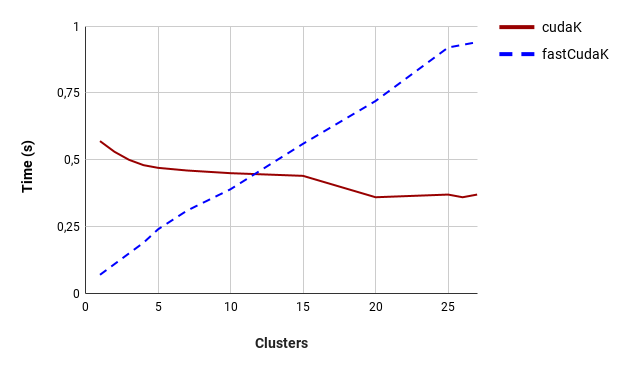
\includegraphics[width=0.5\textwidth]{latex/5.png}
\caption{cudaKmeans Vs fastCudaKmeans with 2 millions pixels, 100 iterations as the number of clusters changes.}
\label{etichetta}
\end{center}
\end{figure}

\begin{table}[H]
\begin{center}
\begin{tabular}{|l|c|c|c|c|}
\hline
Clusters & cudaKmeans & fastCudaKmeans \\
\hline\hline
1 & 0.57 [s] & 0.07 [s] \\
2 & 0.53 [s] & 0.11 [s] \\
3 & 0.5 [s] & 0.15 [s] \\
4 & 0.48 [s] & 0.19 [s] \\
5 & 0.47 [s] & 0.24 [s] \\
7 & 0.46 [s] & 0.31 [s] \\
10 & 0.45 [s] & 0.39 [s] \\
15 & 0.44 [s] & 0.56 [s] \\
20 & 0.36 [s] & 0.72 [s] \\
25 & 0.37 [s] & 0.92 [s] \\
26 & 0.36 [s] & 0.93 [s] \\
27 & 0.37 [s] & 0.94 [s] \\
\hline
\end{tabular}
\end{center}
\caption{Runtimes of cudaKmeans Vs fastCudaKmeans with 2 millions pixels, 100 iterations as the number of clusters changes.}
\end{table}

\begin{figure}[H]
\begin{center}
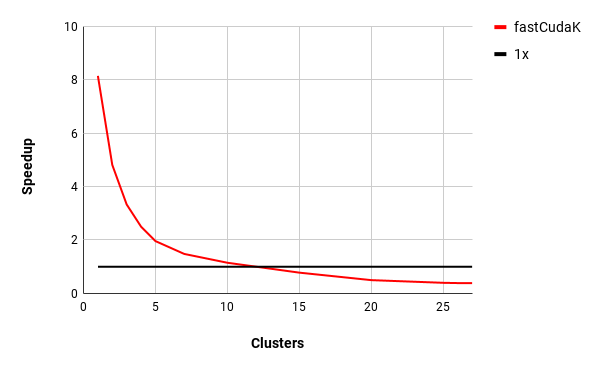
\includegraphics[width=0.5\textwidth]{latex/5s.png}
\caption{Speedup between cudaKmeans and fastCudaKmeans with 2 millions pixels, 100 iterations as the number of clusters changes.}
\label{etichetta}
\end{center}
\end{figure}


\begin{table}[H]
\begin{center}
\begin{tabular}{|l|c|c|c|c|}
\hline
Clusters & Speedup & 1x \\
\hline\hline
1 & 8.14x & 1 \\
2 & 4.81x & 1 \\
3 & 3.33x & 1 \\
4 & 2.5x & 1 \\
5 & 1.96x & 1 \\
7 & 1.48x & 1 \\
10 & 1.15x & 1 \\
15 & 0.78x & 1 \\
20 & 0.5x & 1 \\
25 & 0.4x & 1 \\
26 & 0.39x & 1 \\
27 & 0.39x & 1 \\
\hline
\end{tabular}
\end{center}
\caption{Speedup between cudaKmeans and fastCudaKmeans with 2 millions pixels, 100 iterations respect to number of clusters.}
\end{table}

This test aims to highlight the limits of our algorithm and motivate number of clusters choice for some next tests.

CudaKmeans as the number of clusters increases, it has an initial improvement in performace which stabilizes soon, in fact, after exceeding 20 clusters, times begin to oscillate around the same value. This behavior is justified thanks to the fact that a greater number of clusters means that the number of threads waiting to make the AtomicAdd on a single variable (relative to a cluster) decreases.

On the other hand, fastCudaKmeans algorithm allocates and populates, at each iteration, a quantity of memory directly proportional to both the number of pixels of the image and the number of clusters, we can see how as the latter increase, the performance of fastCudaKmeans worsens almost linearly.

For the reasons just illustrated in some of the next tests, we have chosen a reduced number of clusters so as not to penalize excessively fastCudaKmeans.
\\
The next test compares the execution times of all and all versions, the first graphs vary with the size of the input.

\begin{figure}[H]
\begin{center}
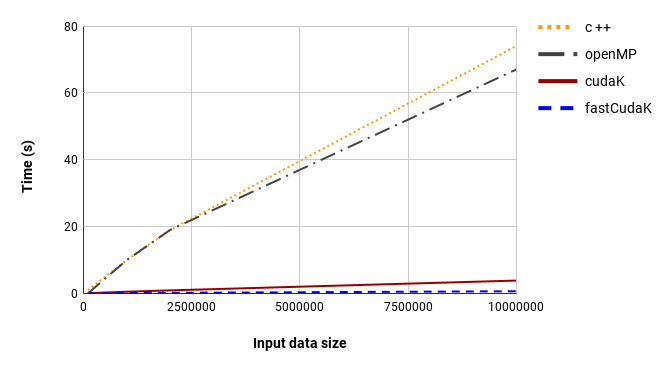
\includegraphics[width=0.5\textwidth]{latex/1.png}
\caption{All versions compared respect to input data size with 2 clusters and 200 iterations.}
\label{etichetta}
\end{center}
\end{figure}

\begin{table}[H]
\begin{center}
\begin{tabular}{|l|c|c|c|c|}
\hline
Data & c++ & openMP & cudaK & fastCudaK\\
\hline\hline
100000 & 1 [s] & 1 [s] & 0.09 [s] & 0.02 [s]\\
1 million & 10 [s] & 10 [s] & 0.54 [s] & 0.13 [s]\\
2 million & 19 [s] & 19 [s] & 0.94 [s] & 0.21 [s]\\
10 million & 74 [s] & 67 [s] & 3.87 [s] & 0.67 [s]\\
\hline
\end{tabular}
\end{center}
\caption{Runtimes of all versions compared respect to input data size with 2 clusters and 200 iterations.}
\end{table}

\begin{figure}[H]
\begin{center}
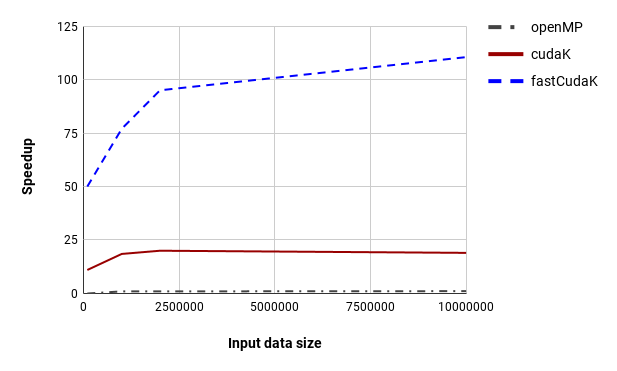
\includegraphics[width=0.5\textwidth]{latex/1s.png}
\caption{Speedup of all versions compared respect to input data size with 2 clusters and 200 iterations.}
\label{etichetta}
\end{center}
\end{figure}

\begin{table}[H]
\begin{center}
\begin{tabular}{|l|c|c|c|c|}
\hline
Data & Speedup omp & Speedup CK & Speedup FCK\\
\hline\hline
100000 & 1x & 11x & 50x \\
1 million & 1x & 18.5x & 77x \\
2 million & 1x & 20x & 95x \\
10 million & 1.1x & 19x & 110.5x\\
\hline
\end{tabular}
\end{center}
\caption{Speedup of all versions compared respect to input data size with 2 clusters and 200 iterations.}
\end{table}

The test shows the differences in performance of the different algorithms. Even if fixing the number of clusters at 2 means creating the best situation for fastCudaKmeans, we still see that by using a reasonable number of clusters we continue to have performance advantages due to the reduction (although the gap between the fastCudaKmeans and cudaKmeans speedup is reduced).


\begin{figure}[H]
\begin{center}
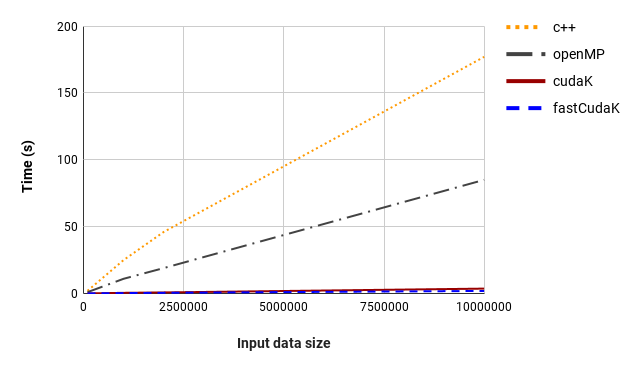
\includegraphics[width=0.5\textwidth]{latex/2.png}
\caption{All versions compared respect to input data size with 7 clusters and 200 iterations.}
\label{etichetta}
\end{center}
\end{figure}

\begin{table}[H]
\begin{center}
\begin{tabular}{|l|c|c|c|c|}
\hline
Data & c++ & openMP & cudaK & fastCudaK\\
\hline\hline
100000 & 2 [s] & 1 [s] & 0.07 [s] & 0.05 [s]\\
1 million & 25 [s] & 11 [s] & 0.51 [s] & 0.31 [s]\\
2 million & 46 [s] & 19 [s] & 0.8 [s] & 0.52 [s]\\
10 million & 177 [s] & 85 [s] & 3.66 [s] & 1.92 [s]\\
\hline
\end{tabular}
\end{center}
\caption{Runtimes of all versions compared respect to input data size with 7 clusters and 200 iterations.}
\end{table}

\begin{figure}[H]
\begin{center}
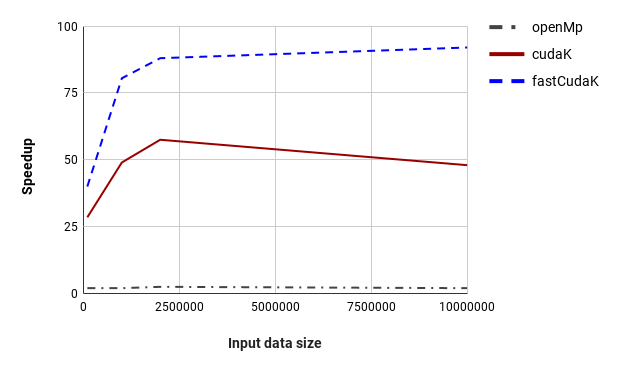
\includegraphics[width=0.5\textwidth]{latex/2s.png}
\caption{Speedup of all versions compared respect to input data size with 7 clusters and 200 iterations.}
\label{etichetta}
\end{center}
\end{figure}

\begin{table}[H]
\begin{center}
\begin{tabular}{|l|c|c|c|c|}
\hline
Data & Speedup omp & Speedup CK & Speedup FCK\\
\hline\hline
100000 & 2x & 28.5x & 40x \\
1 million & 2x & 49x & 80.5x \\
2 million & 2.5x & 57.5x & 88x \\
10 million & 2x & 48x & 92x\\
\hline
\end{tabular}
\end{center}
\caption{Speedup of all versions compared respect to input data size with 7 clusters and 200 iterations.}
\end{table}


We can see how the speedup of cudaKmeans decreases with increasing input because the number of threads waiting for AtomicAdd increases.

These tests also suggest that the openMP version benefits from increasing the number of clusters.
For this reason, now we compare c++ and openMP respect to number of clusters variation.


\begin{figure}[H]
\begin{center}
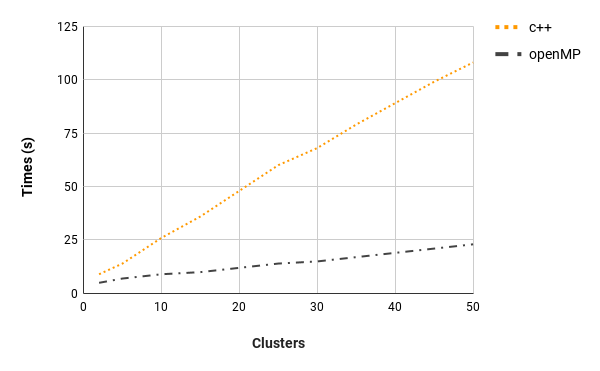
\includegraphics[width=0.5\textwidth]{latex/6.png}
\caption{c++ Vs openMP with 10 millions pixels, 12 clusters as the number of clusters changes.}
\label{etichetta}
\end{center}
\end{figure}


\begin{table}[H]
\begin{center}
\begin{tabular}{|l|c|c|c|c|}
\hline
Clusters & c++ & openMP \\
\hline\hline
2 & 9 [s] & 5 [s] \\
5 & 14 [s] & 7 [s] \\
10 & 26 [s] & 9 [s] \\
15 & 36 [s] & 10 [s] \\
20 & 48 [s] & 12 [s] \\
25 & 60 [s] & 14 [s] \\
30 & 68 [s] & 15 [s] \\
35 & 79 [s] & 17 [s] \\
40 & 89 [s] & 19 [s] \\
45 & 99 [s] & 21 [s] \\
50 & 108 [s] & 23 [s] \\

\hline
\end{tabular}
\end{center}
\caption{Runtimes of c++ Vs openMP with 10 millions pixels, 12 clusters as the number of clusters changes.}
\end{table}

\begin{figure}[H]
\begin{center}
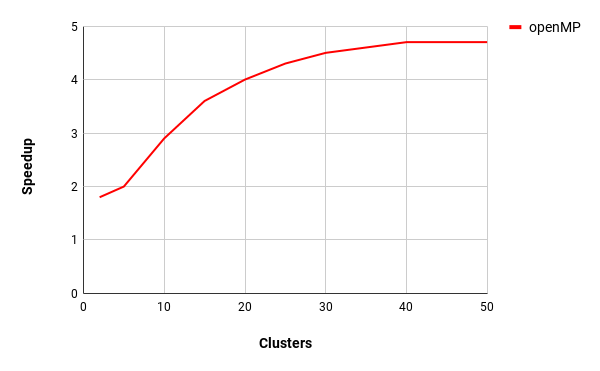
\includegraphics[width=0.5\textwidth]{latex/6s.png}
\caption{Speedup of c++ Vs openMP with 10 millions pixels, 12 clusters as the number of clusters changes.}
\label{etichetta}
\end{center}
\end{figure}



\begin{table}[H]
\begin{center}
\begin{tabular}{|l|c|c|c|c|}
\hline
Clusters & Speedup\\
\hline\hline
2 & 1.8x\\
5 & 2x\\
10 & 2.9x\\
15 & 3.6x\\
20 & 4x\\
25 & 4.3x\\
30 & 4.5x\\
35 & 4.6x\\
40 & 4.7x\\
45 & 4.7x\\
50 & 4.7x\\
\hline
\end{tabular}
\end{center}
\caption{Speedup of c++ Vs openMP with 10 millions pixels, 12 clusters as the number of clusters changes.}
\end{table}

\section{Conclusions}


In conclusion, we think we have focused too much on CUDA details and too little in general algorithm optimization but it is also true that the main purpose of the work was to explore this technology.
Mark Harris suggest to optimize the algorithm first, then unroll loops using template parameters to generate optimal code and we strongly agree with him. Indeed when we ended the test phase we ask ourselves how we could improve the performance changing the algorithm. We would like to maintain the advantages of the reduction but avoiding the redundancy of the population phase. An idea, therefore, would be to reorder the vector of cluster assignments, this makes it possible to maintain a vector of constant size (regardless of number of clusters) and reductions can be made on the values ​​that have same id in the assignment vector, this solution however would have introduced many difficulties related both to the use case (k means) and the common structure of all different implementations.
A new logic should be created to encode information on pixel position relative to image grid in an alternative way, therefore rewrite the ImageHandler and consequently the C ++ versions.
The reduction phase also changes because at each iteration the number of elements to be reduced for each cluster would always be different.
Searching online we found who implemented a kmeans (not with images) using this technique and using Thrust for the reduction and the article in question wanted to demonstrate that in CUDA before optimization it is important to create an intelligent algorithm that exploits the nature of the problem.
However, we think that the field of application of the problem is also important and depending on the intended use of the code,  there is still extensive room for improvement.


{\small
\bibliographystyle{ieee}
\bibliography{egbib}
Optimizing Parallel Reduction in CUDA by
Mark Harris
NVIDIA Developer Technology.
}


\end{document}
